%%%%%%%%%%%%%%%%%%%%%%%%%%%%%%%%%%%%%%%%%%%%%%%%%%%%%%%%%%%%%%%%%%%%%%%%%%%%%%%%
%2345678901234567890123456789012345678901234567890123456789012345678901234567890
%        1         2         3         4         5         6         7         8

%\documentclass[letterpaper, 11 pt, conference]{ieeeconf}  % Comment this line out
                                                          % if you need a4paper
\documentclass[a4paper, 11 pt, conference]{ieeeconf}      % Use this line for a4
                                                          % paper

\IEEEoverridecommandlockouts                              % This command is only
                                                          % needed if you want to
                                                          % use the \thanks command
\overrideIEEEmargins
% See the \addtolength command later in the file to balance the column lengths
% on the last page of the document



% The following packages can be found on http:\\www.ctan.org
%\usepackage{graphics} % for pdf, bitmapped graphics files
%\usepackage{epsfig} % for postscript graphics files
%\usepackage{mathptmx} % assumes new font selection scheme installed
%\usepackage{times} % assumes new font selection scheme installed
%\usepackage{amsmath} % assumes amsmath package installed
%\usepackage{amssymb}  % assumes amsmath package installed

\usepackage[spanish, activeacute]{babel} %Definir idioma español
\usepackage[utf8]{inputenc} %Codificacion utf-8
\usepackage{amsmath}
\usepackage{graphicx}
\usepackage{pifont}% http://ctan.org/pkg/pifont

\usepackage{float}
\usepackage[caption = false]{subfig}
%\usepackage[final]{graphicx}
%\usepackage[export]{adjustbox}
%\usepackage{subcaption}

%\newcommand{\xmult}{\ding{53}}%

\title{\LARGE \bf
Mejora de im\'agenes t\'ermicas a\'ereas basado en morfolog\'ia matem\'atica multiescala con operadores de cambios secuenciales
}

%\author{ \parbox{3 in}{\centering Derlis Gonzalez*
%         \thanks{*Use the $\backslash$thanks command to put information here}\\
%         Faculty of Electrical Engineering, Mathematics and Computer Science\\
%         University of Twente\\
%         7500 AE Enschede, The Netherlands\\
%         {\tt\small h.kwakernaak@autsubmit.com}}
%         \hspace*{ 0.5 in}
%         \parbox{3 in}{ \centering Pradeep Misra**
%         \thanks{**The footnote marks may be inserted manually}\\
%        Department of Electrical Engineering \\
%         Wright State University\\
%         Dayton, OH 45435, USA\\
%         {\tt\small pmisra@cs.wright.edu}}
%}

\author{Derlis Gonz\'alez$^{1}$ % <-this % stops a space
%\thanks{*This work was not supported by any organization}% <-this % stops a space
%\thanks{$^{1}$H. Kwakernaak is with Faculty of Electrical Engineering, Mathematics and Computer Science,
%        University of Twente, 7500 AE Enschede, The Netherlands
%        {\tt\small h.kwakernaak at papercept.net}}%
%\thanks{$^{2}$P. Misra is with the Department of Electrical Engineering, Wright State University,
%        Dayton, OH 45435, USA
%        {\tt\small p.misra at ieee.org}}%
}

\graphicspath{{rsc/}

\begin{document}

\maketitle
\thispagestyle{empty}
\pagestyle{empty}

%%%%%%%%%%%%%%%%%%%%%%%%%%%%%%%%%%%%%%%%%%%%%%%%%%%%%%%%%%%%%%%%%%%%%%%%%%%%%%%%
\begin{abstract}

El mejoramiento de im\'agenes infrarrojas es una t\'ecnica crucial para el mejoramiento de la calidad de im\'agenes infrarrojas. Y, los detalles claros de la imagen son informaciones importantes para el an\'alisis de im\'agenes infrarrojas. Para mejorar efectivamente la imagen infrarroja y hacer claros los detalles de la imagen, un algoritmo basado en operador de cambio secuencial multiescala es propuesto en este paper. Este trabajo presenta una transformada top-hat para el mejoramiento de im\'agenes infrarrojas a\'ereas. El m\'etodo propuesto est\'a basado en el uso de elementos estructurantes incrementales de geometr\'ia similar de operaciones fundamentales de morfolog\'ia matem\'atica. Primeramente, el operador de cambio secuencial, que usa apertura y cerradura como primitivas, es constru\'ido y discutido. Segundo, la extracci\'on caracter\'istica en im\'agenes infrarrojas a trav\'es del operador de cambio secuencial es dado, y la extensi\'on multiescala de la extracci\'on caracter\'istica es discutido en detalle. Finalmente, las caracter\'isticas finales extra\'idas de im\'agenes infrarrojas son constru\'idos e importados en la imagen original infrarroja para producir la imagen mejorada. En la imagen mejorada, las caracter\'isticas de la imagen son bien mejoradas y los detalles de las imagen son claras. Im\'agenes infrarrojas que son obtenidos de diferentes entornos son usados en el experimento. Los resultados muestran que, el algoritmo propuesto es muy efectivo para el mejoramiento de la imagen infrarroja.

\end{abstract}


%%%%%%%%%%%%%%%%%%%%%%%%%%%%%%%%%%%%%%%%%%%%%%%%%%%%%%%%%%%%%%%%%%%%%%%%%%%%%%%%
\section{INTRODUCCI\'ON}

La imagen infrarroja es un tipo de información muy importante en aplicaciones ópticas basadas en infrarrojos, tal como sistema de imagen infrarroja \cite{c1}, sistema de vigilancia infrarroja [2,3] y reconocimiento de objetivo \cite{c4,c6} [4-6]. Sin embargo, debido al efecto del equipamiento de imagen o entorno, la imagen infrarroja obtenida generalmente no es clara y tiene un bajo contraste. Especialmente, en las regiones importantes en im\'agenes infrarrojas donde no sobresale. Eso podr\'ia afectar el an\'alisis de esas im\'agenes. Por lo tanto, el mejoramiento de im\'agenes infrarrojas ser\'ia muy importante.

Actualmente, en muchos casos, la imagen infrarroja que realmente necesita ser mejorada generalmente tiene baja calidad, y el contraste y los detalles de la imagen no son buenas. Por lo tanto, lo crucial de la mejora de la imagen infrarroja es mejorar la imagen y dejar claros los detalles. Para mejorar la imagen infrarroja y detalles, muchos m\'etodos han sido propuestos. Incrementar la resoluci\'on de la imagen es siempre \'util para aplicaciones basadas en im\'agenes [7]. Tambi\'en, modelar el procedimiento f\'isico de la imagen podr\'ia mejorar im\'agenes infrarrojas [8,9]. Pero, si el entorno de la imagen es malo o la distribuci\'on de la imagen es limitada, el rendimiento de esos m\'etodos podr\'ian ser afectados. Mejorar la imagen a trav\'es del efecto visual es efectivo en algunos casos [10,11]. Sin embargo, generalmente necesitan informaci\'on de color, que podr\'ia no ser apropiado para el mejoramiento de im\'agenes infrarrojas con valores de grises. Filtrado de ruido o mejoramiento de eje ha sido usado para mejorar im\'agenes infrarrojas [12]. Pero. el rendimiento no ser\'ia efectivo si la calidad de im\'agenes infrarrojas es baja. A pesar de que los algoritmos basados  en histograma [13-16] son usados ampliamente para el mejoramiento de la imagen, el rendimiento para el mejoramiento de los detalles de la imagen no son buenos. Esto podr\'ia afectar la aplicaci\'on del mejoramiento de la imagen para el an\'alisis y reconocimiento de objetivo. El ajuste de contraste es un modo efectivo para el mejoramiento de la imagen infrarroja [17-19]. Sin embargo, los detalles de la imagen en el mejoramiento de la imagen podr\'ia no ser claros. Morfolog\'ia matem\'atica es una teor\'ia importante en el procesamiento de la imagen [20], que ha sido tambi\'en usado en el procesamiento de la imagen mejorada, incluyendo el mejoramiento de la imagen mejorada [18,20-22].

Mejoramiento de pequeños objetivos en imagen infrarroja es \'util para la detecci\'on de objetivos infrarrojos [21,22]. Pero, no son f\'aciles de ampliar para mejorar otros tipos de im\'agenes infrarrojas. Construir operadores morfol\'ogicos efectivos usando las propiedades de imagen infrarroja es una manera \'util para el mejoramiento de la imagen infrarroja [23]. Pero, algunos detalles de la imagen podr\'ian ser suavizados y el efecto atm\'osfera podr\'ian afectar el rendimiento del algoritmo. En resumen, la mayor\'ia de los algoritmos no pudieron ser efectivamente usado para el mejoramiento de la imagen infrarroja , especialmente para el mejoramiento de los detalles de im\'agenes infrarrojas.

El operador de cambio es un operador morfol\'ogico \'util que podr\'ia identificar detalles de imagen [20,24-26]. Adem\'as, redefiniendo el operador de cambio usando apertura y cerradura como primitivas podr\'ia extraer detalles de im\'agenes [24]. Esto significa que el operador de cambio podr\'ia ser usado para el mantenimiento de los detalles de la imagen mejorada. Por lo tanto, se podr\'ia construir un algoritmo efectivo basado en operador de cambio usando apertura y cerradura como primitivas que podr\'ian mejorar las im\'agenes infrarrojas y detalles de la imagen. 

La transformada top-hat es un m\'etodo importante para el procesamiento de la imagen. Con la transformada top-hat las regiones de brillo y oscuridad son obtenidas, entonces la imagen es mejorada agregando regiones de brillo y removiendo las regiones oscuras de la imagen original \cite{12}, \cite{14}, \cite{15}. El m\'etodo propuesto fue aplicado a im\'agenes infrarrojas a\'ereas una de base de datos de im\'agenes p\'ublicas.

En este trabajo una transformada top-hat es presentado, que usa las operaciones b\'asicas de morfolog\'ia matem\'atica, elementos estructurantes de geometr\'ia similar.

A luz de esto, un algoritmo efectivo para el mejoramiento de im\'agenes infrarrojas basado en operador de cambio secuencial multiescala es propuesto en este paper. Primeramente, se presenta la transformada top-hat propuesto con elementos estructurantes incrementales de geometr\'ia similar. Segundo, el operador de cambio secuencial usando apertura y cerradura como primitivas es mostrado. Tercero, la extracci\'on caracter\'istica a trav\'es de la extensi\'on multiescala es dado en detalle. Finalmente, las caracter\'isticas finales extra\'idas de im\'agenes infrarrojas son calculadas basadas en caracter\'isticas multiescala extra\'idas, y la imagen infrarroja mejorada es producido importando las caracter\'isticas final extra\'idas en la imagen infrarroja final. Las contribuciones principales en este paper son: (1) proponer una transformada top-hat con elementos estructurantes incrementales de geometr\'ia similar; (2) proponer el operador de cambio secuencial; (3) aplicar la extracci\'on de caracter\'isticas para la aplicaci\'on de mejoramiento de imagen infrarroja.

Resultados experimentales en im\'agenes infrarrojas muestran que, las caracter\'isticas de la imagen est\'an mejoradas y los detalles de la imagen son claros. Por lo tanto, el algoritmo propuesto podr\'ia ser usado para el mantenimiento de detalles del mejoramiento de la imagen infrarroja.
\\
\section{MORFOLOG\'IA MATEM\'ATICA}
\\
\subsection{Definiciones b\'asicas}

La mayor\'ia de las operaciones morfol\'ogicas son derivadas de dos operaciones b\'asicas: la dilataci\'on y erosi\'on [20]. La dilataci\'on de la imagen I(x,y) usando elemento estructurante H(u,v) es definido como el m\'aximo de los valores en H agregado a los valores de la subimagen actual de I, representado como  sigue.
$$
I\oplus H = max_{u,v}(I(x-u,y-v) + H(u,v)) 
$$
\( \oplus \) denota la operaci\'on de dilataci\'on, (x,y) y (u,v) son las coordenadas de p\'ixeles en la imagen I y elemento estructurante H, respectivamente. La erosi\'on de la imagen I(x,y) usando el elemento estructurante H(u,v) es definido como el m\'inimo de las diferencias, representado como sigue.
$$
I \ominus H = min_{u,v}(I(x+u,y+v)-H(u,v))
$$

\( \ominus \) denota la  operaci\'on de erosi\'on. \\
Apertura y cerradura, que son las combinaciones de la dilataci\'on y erosi\'on a trav\'es de diferentes modos, son definidos como sigue.

$$
I \circ H = (I \ominus H) \oplus H,
$$
$$
I \bullet H = (I \oplus H) \ominus H.
$$
$ \circ $ y $ \bullet $ representan las operaciones de apertura y cerradura, respectivamente.
La apertura y cerradura son usualmente usados para suavizar brillo y regiones oscuras, respectivamente. Esta propiedad podr\'ia ser usado para la extracci\'on de caracter\'isticas.

\subsection{Transformada Top-hat}
La transformada top-hat originalmente propuesto en \cite{20} provee una herramienta excelente para la extracci\'on de caracter\'isticas de brillos y oscuridad respectivamente m\'as pequeño que un tamaño dado de un fondo desigual.

Usando apertura y cerradura, la transformada top-hat, incluyendo la transformada top-hat por apertura y transformada top-hat por cerradura, denotado por THA y THC, son definidos como sigue, respectivamente \cite{17}.
$$
THA = I - I \circ H
$$

$$
THC = I - H \bullet I
$$

La apertura suaviza regiones de brillos de la imagen y cerradura suaviza regiones oscuras. Por lo tanto, THA descubre regiones de brillo y THC provee regiones oscuras en I \cite{11}.

\subsection{Operador de cambio con apertura y cerradura como primitivas}

El operador de cambio ha sido una herramienta \'util en aplicaciones de procesamiento de imagen despu\'es que ha sido propuesto [20,24,25]. Primitivas y reglas son dos factores principales en el operador de cambio. Suponga $ I_1(x,y) $ y $ I_2(x,y) $ son las primitivas, un tipo de operador de cambio es definido como sigue [20,24,25].

\begin{equation} \label{exp:exp1}
\begin{tiny}
\centering
%%\[ 
OC(I)(x,y) = 
    \begin{cases}
     I_1(x,y), \quad \text{if }   I_2(x,y)-I(x,y) < I(x,y)-I_1(x,y) \\ 
     I_2(x,y), \quad \text{if }  I_2(x,y)-I(x,y) > I(x,y)-I_1(x,y)  \\
    I(x,y), \quad \text{else }
    \end{cases}
%%\]
\end{tiny}
\end{equation}

\normalsize
La selecci\'on de reglas en este operador de cambio indica, este operador extrae los p\'ixeles de im\'agenes que son mas diferentes de la imagen original I en las primitivas $ I_1(x,y) $ y $ I_2(x,y) $. Esos p\'ixeles de la imagen generalmente representan caracter\'isticas importantes en la imagen. Por lo tanto, este tipo de operador de cambio ser\'ia \'util para la extracci\'on de caracter\'isticas.

La definici\'on de las primitivas en OC afecta el rendimiento del OC para la extracci\'on de caracter\'isticas. La apertura y cerradura son operadores efectivos para suavizar im\'agenes caracter\'isticas. Usando apertura y cerradura como primitivas en OC ser\'ia \'util para la extracci\'on de caracter\'isticas importantes [24]. Esto es efectivo para identificar los detalles de im\'agenes infrarrojas. El operador de cambio usando apertura y cerradura como primitivas ser\'ia expresado como sigue [24].

\tiny 
\begin{equation} \label{eq:operadorcambio}
 \centering    
 OC(I)(x,y) = 
    \begin{cases}
    I \circ H(x,y), \quad \text{if } I \bullet H(x,y)-I(x,y) < I(x,y)-I \circ H(x,y) \\
     I \bullet H(x,y), \quad \text{if } I \bullet H(x,y)-I(x,y) > I(x,y)-I \circ H(x,y) \\
    I(x,y), \quad \text{else }
    \end{cases}

\end{equation}
\normalsize
En esta definici\'on, la diferencia entre la imagen original y el resultado de la apertura o cerradura es comparada. Y, los p\'ixeles en el resultado del OC son del resultado de la apertura o cerradura. Cada pixel tiene una diferencia relativamente m\'as grande que la imagen original y el resultado de la apertura o cerradura. Una gran diferencia indica que el suavizamiento de las caracter\'isticas de la imagen por apertura o cerradura son mas sobresaliente en la imagen.

Esas caracter\'isticas son caracter\'isticas importantes en la imagen. Por lo tanto, esta definici\'on de OC ser\'ia \'util para la extracci\'on de caracter\'isticas.

Actualmente, las caracter\'isticas de im\'agenes importantes en la imagen infrarroja son generalmente regiones sobresalientes en comparaci\'on con otras regiones. Y, mejorar la imagen infrarroja ser\'ia mejorar las caracter\'isticas de la imagen que son diferentes de otras regiones. OC en la expresi\'on \eqref{exp:exp1} ser\'ia usado para extraer caracter\'isticas que sobresale en la imagen. Por lo tanto, la definici\'on de OC en la expresi\'on \eqref{exp:exp1} ser\'ia usado para el mejoramiento de im\'agenes infrarrojas.
\\
\section{MEJORAMIENTO DE IMAGEN INFRARROJA}
\subsection{Construcci\'on de la transformada top-hat con dos elementos estructurantes}

La idea principal es aplicar la transformada top-hat, usando elementos estructurantes de geometr\'ia similar con diferentes escalas. Trabajos recientes que hacen uso de diferentes elementos estructurantes en la transformada top-hat existente en la literatura, no retiene la geometr\'ia exacta de los elementos estructurantes \cite{18},\cite{19}.

Se define EE un elemento estructurante convexo, (n - 1) el n\'umero dilataciones para $EE_n$ en un rango de \textit{i} = 1,2, ... n y (m - 1) es el n\'umero de dilataciones para $EE_m$ en un rango de \textit{j} = 1,2, ... m, como sigue:

$$
EE_n = EE_{n-1} \oplus EE = \underbrace{EE \oplus EE \oplus EE \oplus ... \oplus EE}_\text{n - 1 dilataciones}
$$

$$
EE_m = EE_{m-1} \oplus EE = \underbrace{EE \oplus EE \oplus EE \oplus ... \oplus EE}_\text{m - 1 dilataciones}
$$

Por lo tanto, definimos los elementos estructurantes $H_1$ y $H_2$ como sigue:

\begin{equation} \label{eq:h1}
H_1 = EE_n    
\end{equation}

\begin{equation} \label{eq:h2}
H_2 = EE_m
\end{equation}

Donde $H_1$ y $H_2$ son planos y geom\'etricamentes proporcionales, debido a que la base del elemento estructurante EE es convexo.

Considerando los elementos estructurantes incrementales, la transformada top-hat se define como:

\begin{equation} \label{eq:th1}
THAN = I - ((I \ominus H_1) \oplus H_2)
\end{equation}

\begin{equation} \label{eq:th2}
THCN = ((I \oplus H_1) \ominus H_2) - I    
\end{equation}


\subsection{Construcci\'on del operador de cambio secuencial} 
La imagen contiene caracter\'isticas en diferentes escalas. Extraer caracter\'isticas multiescala ser\'ia efectivo para el procesamiento de imagen. En morfolog\'ia matem\'atica, usar elementos estructurantes multiescala con tamaños incrementales es una buena manera de extraer caracter\'isticas multiescala [23,24,26-28]. 

Suponga \eqref{eq:h1} y \eqref{eq:h2}, elementos estructurantes multiescala con tamaños incrementales. 
$$ 
H_i = \underbrace{H_i \oplus H_1 ... \oplus H_1 }_\text{dilataci\'on i veces}, 1 \leq i \leq n 
$$ 
$$ 
H_j = \underbrace{H_j \oplus H_1 ... \oplus H_1 }_\text{dilataci\'on j veces}, 1 \leq j \leq m 
$$ 

Basado en esos elementos estructurantes multiescala, el operador de cambio secuencial ser\'ia definido como sigue.
$\\\\
OC_i(I) = OC_i(OC_{i-1}(I)).
$
$\\
OC_0(I) = I.\\\\
$
Una ilustraci\'on del operador de cambio secuencial $OC_i$ usando los elementos estructurantes multiescala se muestra en la Fig. \eqref{fig:Fig. 1}. 

\begin{figure}
    \centering
    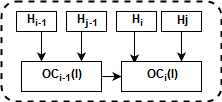
\includegraphics[width=6.5cm,height=2cm,angle=0]{rsc/TOGF.png}
    \caption{Una ilustraci\'on del operador de cambio secuencial usando $OC_i$.}
    \label{fig:Fig. 1}
\end{figure}

En esta definici\'on, el operador de cambio secuencial usa elementos estructurantes para secuencialmente procesar caracter\'isticas de la imagen correspondiente a diferentes escalas. Por lo tanto, bas\'andose en el operador de cambio secuencial, la existencia de caracter\'isticas de imagen en diferentes escala podr\'ia ser identificado. Entonces, las caracter\'isticas de imagen de cada escala ser\'ia para el an\'alsis de la imagen. Esto ser\'ia \'util para el mejoramiento de imagen infrarroja.
Las regiones importantes en la imagen infrarroja son generalmente caracter\'isticas brillosas u oscuras que son diferentes de otras regiones. Por lo tanto, ser\'ia significativa para el mejoramiento de imagen infrarroja para extraer y utilizar las caracter\'isticas multiescala contenida de la imagen infrarroja original.

\subsection{Extracci\'on de caracter\'isticas basada en operador de cambio secuencial}

$OC_i(I)$ secuencialmente suaviza las caracter\'isticas de la imagen en las escalas de 1 a i. $OC_{i-1}(I)$ secuencialmente suaviza las caracter\'isticas de la imagen en las escalas de 1 a i - 1. Entonces, las caracter\'isticas de la imagen suavizado por el operador de cambio secuencial correspondiente a la escala i ser\'ia extra\'ido comparando $OC_i(I) $ con $OC_{i-1}(I)$.
El resultado del operador de cambio secuencial suaviza caracter\'isticas de imagen brillosas y oscuras. $OC_{i-1}(I)$ suaviza las caracter\'isticas de imagen oscura y brillosas en las escalas de 1 a i - 1. $OC_i(I)$ suaviza las caracter\'isticas de imagen brillosas y oscuras en las escala de 1 a i. Los valores grises de las caracter\'isticas de imagen suavizadas ser\'a deprimido por el operador de cambio secuencial. Por lo tanto, comparando los valores grises de $OC_i(I)$ y $OC_{i-1}(I)$, las caracter\'isticas brillosas suavizadas en la escala i ser\'ia extra\'ido por el operador de cambio secuencial. Actualmente, la estrategia de comparaci\'on entre pixeles ha sido verificada como una manera efectiva de extracci\'on de caracter\'isticas de im\'agenes basada en operadores morfol\'ogicas [18,20-26]. Esta estrategia podr\'ia ser tambien usado en este paper por el operador de cambio secuencial para la extracci\'on de caracter\'isticas, que ser\'ia expresado como sigue.
\begin{small}


$$
BCOCS_i(I)(x,y) = max(OC_{i-1}(x,y) - OC_i(I)(x,y),0).
$$

\end{small}
$BCOCS_i(I)$ es las caracter\'isticas brillosas extra\'idas en la escala i usando el operador de cambio secuencial.
Similarmente, $OC_{i-1}(I) $ suaviza las caracter\'isticas de imagen oscuras en las escala de 1 a i - 1. $OC_i(I)$ suaviza las caracter\'isticas de image oscuras en la escala de 1 a i. Los valores grises de las caracater\'isticas de imagen oscuras son pequeñas. Entonces, los valores grises en las caracter\'isticas de la imagen oscuras suavizadas ser\'a incrementada por TO. Por lo tanto, comparando los valores grises de $OC_i(I)$ y $OC_{i-1}(I)$, las caracter\'isticas oscuras suavizadas en la escala i ser\'ia extra\'ida por el operador de cambio secuencial como sigue.

\begin{small}
$$
OCOCS_i(I)(x,y) = max(OC_i(x,y) - OC_{i-1}(I)(x,y),0).
$$

\end{small}

Variando la escala i, las caracater\'isticas de imagen efectiva identificada por el operador de cambio secuencial en diferentes escalas ser\'ia extra\'ida. Esas caracter\'isticas de imagen son principalmente extra\'idas basadas en valores de gris, que corresponde a las caracter\'isticas efectivas en imagen infrarroja. Por lo tanto, esas caracter\'isticas extra\'idas ser\'ia muy \'util para el mejoramiento de la imagen infrarroja.

\subsection{Extracci\'on final para mejoramiento}

Las caracter\'isticas de brillo final $BCOCS_i(I)$ solo contiene las caracter\'isticas de imagen correspondiente a la escala i. Agregar  caracter\'isticas de imagen multiescala ha sido una manera efectiva para extracci\'on de caracter\'isticas en diferentes aplicaciones [18,20,22-26]. As\'i, las caracter\'isticas de brillo extra\'ido de diferentes escalas (denotado por FBCOCSA) por el operador de cambio secuencial en este paper podr\'ia ser tambi\'en efectivamente combinado a trav\'es de la suma entre p\'ixeles de $BCOCS_i(I)$ de todas las escalas como sigue.

$$
FBCOCSA(x,y) = \sum_{i} [BCOCS_i(x,y)].
$$

Adem\'as, las caracter\'isticas de brillo extra\'ida de imagen infrarroja usualmente tienen valores de grises grandes en $BCOCS_i(I)$. Entonces, las caracter\'isticas de brillo importante, que usualmente representa los detalles de la imagen, tendr\'ia los valores de grises m\'as grandes en todas las escalas. Adem\'as, la operaci\'on de m\'aximo entre pixeles, que ha sido efectivamente usado por otros operadores morfol\'ogicas para la extracci\'on de caracter\'isticas de imagen importantes [18-26], ser\'ia tambien usado en este paper por el operador de cambio secuencial para la extracci\'on de brillo caracter\'isticos importantes. Por lo tanto, las caracter\'isticas de brillos importantes (denotado por FBCOCSM) ser\'ia obtenido aplicando la operaci\'on de m\'aximo entre pixeles en $BCOCS_i(I)$ de todas las escalas como sigue.

$$
FBCOCSM(x,y) = max_i[BCOCS_i(x,y)].
$$

Para mejorar las caracter\'isticas de brillo de la imagen, especialmente los detalles de brillo de la imagen, las caracter\'isticas de brillo importante extra\'ida FBCOCSM podr\'ia ser agregado en FBCOCSA. Por lo tanto, las caracter\'isticas de brillo final extra\'ido de im\'agenes infrarrojas ser\'ia la combinaci\'on de las caracter\'isticas de brillo extra\'idas de todas las escalas como sigue.

$$FBCOCS = FBCOCSA + FBCOCSM$$.

FBCOCS representa las caracter\'isticas final de brillo extra\'ida de imagen infrarroja a trav\'es del operador de cambio secuencial, que podr\'ia ser usado para el mejoramiento de las caracter\'isticas de brillo de imagen, especialmente el mejoramiento de los detalles brillosas de la imagen.

De manera similar, debido a que las caracter\'isticas oscuras extra\'idas  $OCOCS_i(I)$ solo contiene las caracter\'isticas de imagen correspondiente a la escala i, las caracter\'isticas oscuras extra\'idas de diferentes escalas (denotado por FOCOCSA) podr\'ia ser combinado a trav\'es de la sumatoria entre pixeles de $OCOCSA_i(I)$ de todas las escalas como sigue.

$$
FOCOCSA(x,y) = \sum_{i} [OCOCS_i(x,y)].
$$

Adem\'as, las caracter\'isticas oscuras extra\'idas de imagen infrarroja tienen grandes valores de grises en $OCOCS_i(I)$. Entonces, las caracter\'isticas de imagen oscuras importantes, que usualmente representa los detalles de la imagen oscura, tendr\'ia los valores de grises mas grandes en todas las escalas. Por lo tanto, las caracter\'isticas oscuras importantes (denotado por FOCOCSM) podr\'ia ser obtenido por la operaci\'on de m\'aximo en $OCOCS_i(I)$ de todas las escalas como sigue.

$$
FOCOCSM(x,y) = max_i[OCOCS_i(x,y)].
$$

Para mejorar las caracter\'isticas de oscuras de la imagen, especialmente los detalles oscuros de la imagen, las caracter\'isticas oscuras importante extra\'ida FOCOCSM podr\'ia ser agregado en FOCOCSA. Por lo tanto, las caracter\'isticas oscuras final extra\'ido de im\'agenes infrarrojas ser\'ia la combinaci\'on de las caracter\'isticas oscuras extra\'idas de todas las escalas como sigue.

$$FOCOCS = FOCOCSA + FOCOCSM$$.

FDFSTO representa las caracter\'isticas final oscuras extra\'ida de imagen infrarroja a trav\'es del operador de cambio secuencial, que podr\'ia ser usado para el mejoramiento de las caracter\'isticas oscuras de imagen, especialmente el mejoramiento de los detalles oscuras de la imagen.

%%Un ejemplo de la extracci\'on de caracter\'isticas es mostrado en Fig.2.(a) es la imagen original infrarroja. (b) y (c) son las caracter\'isticas de brillo y oscuridad final extra\'idas de la imagen infrarroja, respectivamente. Los valores de grises de la Fig.2(b) y (c) son ajustado dentro del intervalo de grises [1,70] para claramente mostrar las caracter\'isticas de brillo y oscuridad. Fig. 2(b) y (c) muestra que, esas caracter\'isticas final extra\'idas representa la regiones importantes de brillo y oscuridad y detalles de la imagen original infrarroja.
%%Especialmente, Fig. 2(b) contiene las caracter\'isticas importantes de la regi\'on objetiva. Por lo tanto, esas caracter\'isticas podr\'ia ser usado para mejorar la imagen infrarroja original efectivamente.

\subsection{Mejoramiento de la imagen infrarroja}

Una manera efectiva de mejoramiento de la imagen infrarroja es mejorar los detalles de la imagen a trav\'es de la ampliaci\'on de contraste de la imagen infrarroja original [23]. FBCOCS es la caracter\'istica de brillo final extra\'ida de la imagen infrarroja por el operador de cambio secuencial, y FOCOCS es la caracter\'istica oscuras final extra\'ida. Entonces, siguiendo la ampliaci\'on de contraste [23], el contraste de la imagen infrarroja original podr\'ia ser ampliada como sigue. 

$$
I_{ME} = p_1  *  I + p_2 * FBCOCS - p_3 * FOCOCS
$$

$I_{ME}$ representa la imagen infrarroja final mejorada, $p_1$, $p_2$ y $p_3$ son los pesos para ajustar el contraste del resultado de la imagen.

FBCOCS y FOCOCS son las caracter\'isticas final de brillo y oscuridad respectivamente. Importando esas caracter\'isticas de imagen que contiene los detalles de la imagen en la imagen infrarroja original podr\'ia mejorar los detalles de la imagen en la imagen infrarroja. Tambien, el contraste de las caracter\'isticas de brillo y oscuridad son ampliadas a trav\'es del mejoramiento de contraste. Adem\'as, el contraste del resultado de la imagen final  podr\'ia ser ajustado a trav\'es de los pesos para obtener un resultado de mejoramiento efectivo. Por lo tanto, el contraste y los detalles de imagen de la imagen infrarroja original son mejoradas, lo que resulta en un resultado efectivo del mejoramiento de la imagen infrarroja.

\begin{figure}
    %\centering
    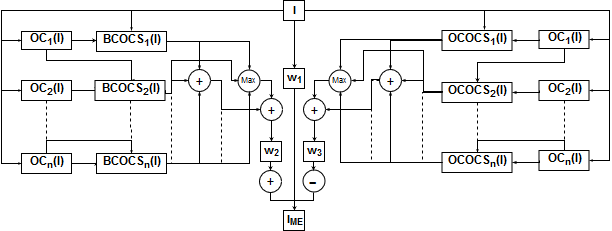
\includegraphics[width=8.8cm,height=3.5cm,angle=0]{rsc/AP.png}
    \caption{El procedimiento del algoritmo propuesto}
    \label{fig:Fig. 2}
\end{figure}

El procedimiento del algoritmo propuesto se muestra en la Fig. 2. Primeramente, las caracter\'isticas de brillo y oscuridad multiescala de la imagen infrarroja son extra\'idas. Segundo, las caracter\'isticas final de brillo y oscuridad son calculadas desde las caracter\'isticas de brillo y oscuridad multiescala extra\'idas. Finalmente, la imagen infrarroja es mejorada usando el modo de ampliaci\'on de contraste. Fig. 4 muestra el resultado final del mejoramiento de la imagen infrarroja original en la Fig. 1(a). Fig. 4 indica que, la imagen y los detalles son mejorados efectivamente. Y, el objetivo es m\'as claro que la imagen infrarroja original. Este resultado mejorado beneficiar\'ia el an\'alisis posterior de la imagen infrarroja.

\subsection{Selecci\'on de par\'ametros}

El elemento estructurante es un par\'ametro importante en el algoritmo propuesto.
El elemento estructurante ampliamente utilizado es un elemento estructurante plano. En el elemento estructurante plano, solo el tamaño y la forma del elemento estructurante ser\'ia decidido. Por lo tanto, si la forma y tamaño fueran decididos, entonces el elemento estructurante usado en cada escala corresponde al n\'umero de la escala.  En este caso, el par\'ametro principal del elemento estructurante plano que ser\'ia decidido es la forma del elemento estructurante. La forma circular ha sido ampliamente utilizado en diferentes aplicaciones [20]. Y, no hay esquinas agudas en el circulo, que podr\'ia suprimir algunos efectos de bloques. As\'i, la forma circular es usado en este paper. Por lo tanto, el elemento estructurante usado en este paper es el elemento estructurante plano con forma circular.

El n\'umero de escala n determina las caracter\'isticas de las im\'agenes extra\'idas. Usando n\'umero de escala grande podr\'ia extraer m\'as caracter\'isticas de imagen. Generalmente, no hay necesidad de extraer caracter\'isticas de imagen en escala muy alta debido a que los detalles de la imagen infrarroja en escalas altas no son muy ricos [23]. Entonces, no hay necesidad de usar numeros de escalas grandes. Los resultados experimentales en im\'agenes infrarrojas muestran que, usando n\'umero de escala entre [3,7] es efectivo para la mayor\'ia de las im\'agenes. En este paper, usamos n\'umero de escala n = 5. Y, los resultados experimentales verific\'o que usando n = 5 fue efectivo para el mantenimiento del mejoramiento de los detalles de la imagen infrarroja.

Los valores de los pesos $p_1$, $p_2$, $p_3$ son usados para el ajustar el contraste del mejoramiento final de la imagen infrarroja y as\' mejorar aun m\'as los detalles de la imagen. Generalmente, hay valores positivos entre [0,3]. Para mejorar bien las caracter\'isticas de la imagen extra\'ida y obtener un buen contraste, $p_1$ ser\'ia pequeño, y $p_2$ y $p_3$ ser\'ia grande. En este paper, definimos $p_1$ = 0.6, $p_2$ = 1.5 y $p_3$ = 1.5. Los resultados experimentales verific\'o que, esos pesos fueron efectivos.

\section{Resultados experimentales}

Para verificar el rendimiento efectivo del algoritmo propuesto, im\'agenes infrarrojas con diferentes tipos de desorden de fondos y obtenidos bajo diferentes circunstancias son usados en este experimento. Para ser una comparaci\'on justa, el conjunto de datos usados de las im\'agenes infrarrojas originales es el mismo que [23]. Adem\'as, algunos algoritmos podr\'ian ser usados para mejoramiento de im\'agenes infrarrojas, incluyendo el algoritmo de ecualizaci\'on de histograma (HE)[15,16], algoritmo de equalizaci\'on  de histograma de contraste adaptativo limitado (CLAHE) [16],  y algoritmo basado en operador de cambio secuencial multiescala (MSSTO) [23], son usados en este paper como algoritmos de comparaci\'on. HE y CLAHE son algoritmos ampliamente usados para mejoramiento de imagen, que podr\'ian ser usado para el mejoramiento de la imagen infrarroja. MSSTO es un algoritmo efectivo para el mejoramiento de imagen infrarroja, que tambi\'en est\'a basado en la teor\'ia de la matem\'atica morofol\'ogica multiescala con operador de cambio secuencial y podr\'ia ser usado para el mejoramiento bien de la imagen infrarroja. Por lo tanto, HE, CLAHE, MSSTO son adoptados en este paper para hacer la comparaci\'on. Los experimentos de comparaci\'on cuantitativa y visual son mostrados abajo.

\begin{figure}
    \centering
    \subfloat[]{
        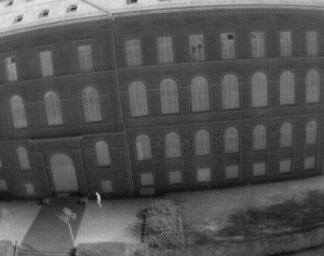
\includegraphics[width = 0.25\textwidth]{rsc/res1/520.png}
    } \\
    \subfloat[]{
        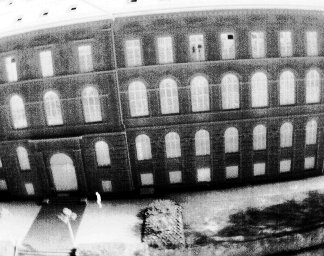
\includegraphics[width = 0.25\textwidth]{rsc/res1/520HE.png}
    }
    \subfloat[]{
        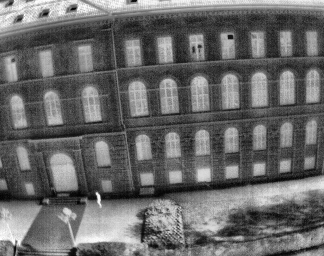
\includegraphics[width = 0.25\textwidth]{rsc/res1/520CLAHE.png}
    }\\
    \subfloat[]{
        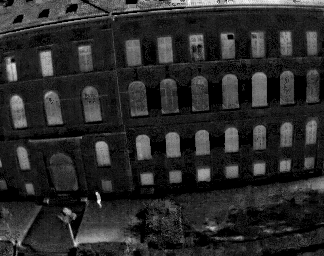
\includegraphics[width = 0.25\textwidth]{rsc/res1/520PAPER.png}
    }
    \subfloat[]{
        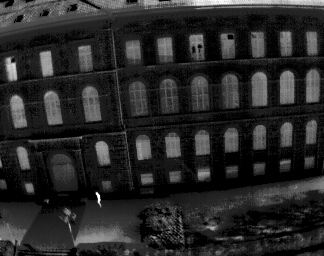
\includegraphics[width = 0.25\textwidth]{rsc/res1/520PROP.png}
    } 
    \caption{Un ejemplo de comparaci\'on de im\'agenes infrarrojas (a) la imagen original (b) es el resultado mejorado de HE (c) es el resultado mejorado de CLAHE (d) es el resultado mejorado de MSSTO (e) es el resultado mejorado del algoritmo propuesto.}
    \label{fig:fig3}

\end{figure}

%\begin{figure}[h]
%\centering
%\begin{minipage}{0.4\textwidth}%
%\subfloat[Subfigure 1 list of figures text][Subfigure 1 caption]{
%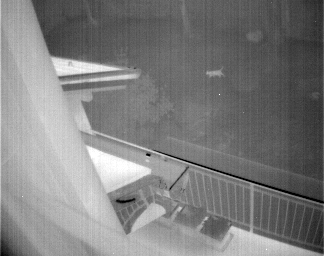
\includegraphics[width=0.4\textwidth]{rsc/res3/44.png}
%\label{fig:subfig1}}
%\end{minipage}%
%\begin{minipage}{0.4\textwidth}%
%\subfloat[Subfigure 1 list of figures text][Subfigure 1 caption]{
%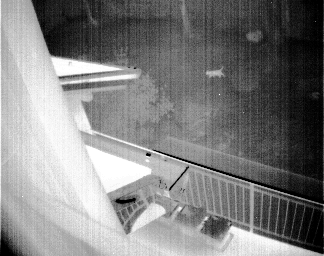
\includegraphics[width=0.4\textwidth]{rsc/res3/44HE.png}
%\label{fig:subfig1}}
%\end{minipage}%
%\qquad
%\begin{minipage}{0.4\textwidth}%
%\subfloat[Subfigure 2 list of figures text][Subfigure 2 caption]{
%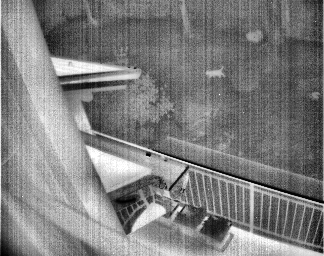
\includegraphics[width=0.4\textwidth]{rsc/res3/44CLAHE.png}
%\label{fig:subfig2}} \\
%\subfloat[Subfigure 3 list of figures text][Subfigure 3 caption]{
%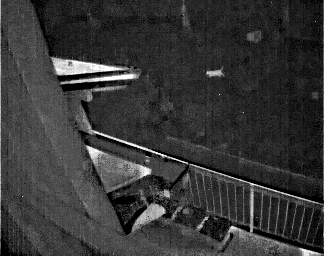
\includegraphics[width=0.4\textwidth]{rsc/res3/44PAPER.png}
%\label{fig:subfig3}}
%\end{minipage}
%\begin{minipage}{0.4\textwidth}%
%\subfloat[Subfigure 1 list of figures text][Subfigure 1 caption]{
%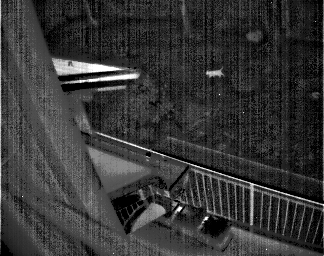
\includegraphics[width=0.4\textwidth]{rsc/res3/44PROP.png}
%\label{fig:subfig1}}
%\end{minipage}%

%\caption{This is a figure containing several subfigures.}
%\label{fig:globfig}
%\end{figure}


\begin{figure}
    \centering
    \subfloat[]{
        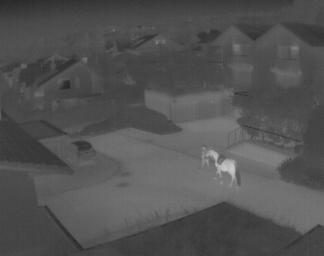
\includegraphics[width = 0.23\textwidth]{rsc/res2/306.png}
    } \\
    \subfloat[]{
        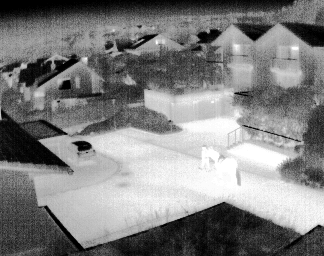
\includegraphics[width = 0.23\textwidth]{rsc/res2/306HE.png}
    }
    \subfloat[]{
        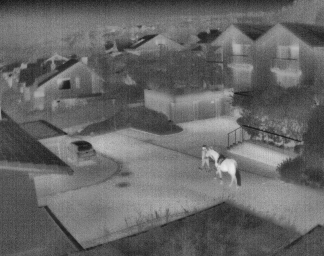
\includegraphics[width = 0.23\textwidth]{rsc/res2/306CLAHE.png}
    }\\
    \subfloat[]{
        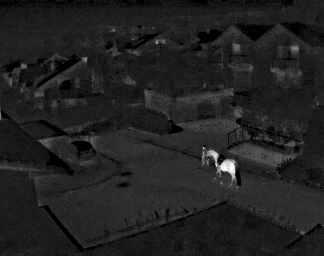
\includegraphics[width = 0.23\textwidth]{rsc/res2/306PAPER.png}
    }
    \subfloat[]{
        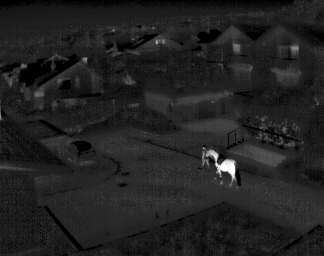
\includegraphics[width = 0.23\textwidth]{rsc/res2/306PROP.png}
    } 
    \caption{Un ejemplo de comparaci\'on de im\'agenes infrarrojas (a) la imagen original (b) es el resultado mejorad de HE (c) es el resultado mejorado de CLAHE (d) es el resultado mejorado de MSSTO (e) es el resultado mejorado del algoritmo propuesto.}
    \label{fig:fig4}

\end{figure}

\begin{figure}
    \centering
    \subfloat[]{
        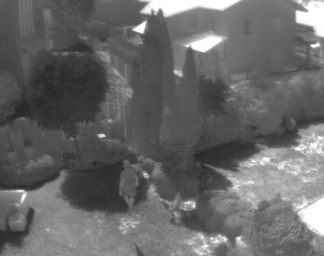
\includegraphics[width = 0.23\textwidth]{rsc/res4/90.png}
    } \\
    \subfloat[]{
        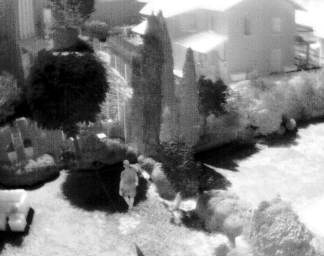
\includegraphics[width = 0.23\textwidth]{rsc/res4/90HE.png}
    }
    \subfloat[]{
        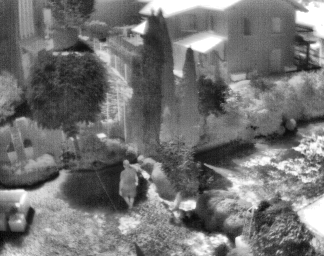
\includegraphics[width = 0.23\textwidth]{rsc/res4/90CLAHE.png}
    }\\
    \subfloat[]{
        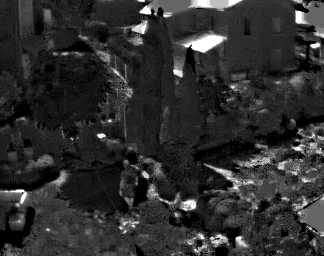
\includegraphics[width = 0.23\textwidth]{rsc/res4/90PAPER.png}
    }
    \subfloat[]{
        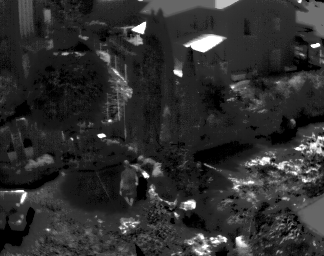
\includegraphics[width = 0.23\textwidth]{rsc/res4/90PROP.png}
    } 
    \caption{Un ejemplo de comparaci\'on de im\'agenes infrarrojas (a) la imagen original (b) es el resultado mejorad de HE (c) es el resultado mejorado de CLAHE (c) es el resultado mejorado de MSSTO (d) es el resultado mejorado del algoritmo propuesto.}
    \label{fig:fig5}

\end{figure}

\subsection{Comparaci\'on visual}

Fig. \eqref{fig:fig3} es un ejemplo de comparaci\'on en la imagen infrarroja con objetivos a\'ereos y fondos desordenados. (a) es la imagen infrarroja original \textit{590.png}. (b) es el resultado mejorado de HE. (c) es el resultado mejorado de CLAHE. (d) es el resultado mejorado de MSSTO. (e) es el resultado mejorado del algoritmo propuesto. La imagen original no tiene un buen contraste y la imagen no est\'a clara. Los resultados mejorados de HE y CLAHE mejora las regiones de brillo de la imagen original. Pero, las regiones a\'ereas no es clara en comparaci\'on con la imagen original. Adem\'as, los ruidos son pesados en esos resultados. MSSTO mejora la imagen infrarroja, pero los ruidos de la imagen mejorada son tambien pesados. El resultado de MSNTH tiene buen  contraste y el objetivo es brilloso. Pero, las alas de las naves no est\'an bien mejorados. El algoritmo propuesto mejora la imagen original. En la imagen mejorada, el contraste es bueno y los ruidos contenidos son pocos. Adem\'as, la regi\'on completa de la nave objetivo es mejorada, incluyendo las alas. Por lo tanto, el algoritmo propuesto realiza mejor que otros algoritmos.

Fig. 6 es un ejemplo de comparaci\'on en imagen infrarroja con objetivo en la nave y fondos de cielo y mar desordenados. (a) es la imagen infrarroja original. (b) es el resultado mejorado de HE. (c) es el resultado mejorado de CLAHE. (d) es el resultado mejorado de MSM. (e) es el resultado mejorado de MSNTH. (f) es el resultado mejorado del algoritmo propuesto. Debido a la niebla atmosf\'erica, la imagen infrarroja original no es clara y los objetivos no son claros. Por lo tanto, la distribuci\'on de grises de la imagen infrarroja original est\'a limitada. HE sobremejora las regiones objetivas y algun desorden del fondo del oc\'eano. Y, un objetivo muy oscuro podr\'ia no ser observado en el resultado mejorado.  CLAHE mejora la imagen completa, pero las regiones objetivas aun no son claras. MSM mejora la imagen original, y las regiones objetivas son claras. Sin embargo, muchos ruidos son producidos en la imagen resultado. MSNTH mejora el contraste de la imagen. Las regiones objetivasson claras y hay pocos ruidos en el resultado. Sin embargo, los detalles de la imagen en el fondo del oc\'eano y cielo no son claros. El algoritmo propuesto mejora la imagen original y las regiones objetivas.

El contraste de la imagen resultante es buena. Tambien, las regiones objetivas son claras, y los detalles de la imagen son preservados. Sin embargo, los ruidos son menos que el resultado de MSM. Por lo tanto, el algoritmo propuesto realiza mejor que otros algoritmos.

Fig. 7 es un ejemplo de comparaci\'on en imagen infrarroja con objetivos de naves oscuras y fondo de oc\'eano desordenado. (a) la imagen infrarroja original. (b) es el resultado mejorado de HE. (c) es el resultado mejorado de CLAHE. (d) es el resultado mejorado de MSM. (e) es el resultado mejorado de MSNTH. (f) es el resultado mejorado del algoritmo propuesto. El objetivo en la imagen original es muy negra. Y, la imagen original no es clara. HE sobremejora las regiones del cielo. Por lo tanto, las regiones objetivas de las naves alrededor de la parte baja de la regi\'on del cielo esta mas invisible. CLAHE mejora la imagen completa. 

Pero, algunas regiones desordenados del oc\'eano en la parte baja de la imagen est\'an sobremejorados. Por lo tanto, la nave objetiva no es muy clara. MSM mejora la imagen original y la regi\'on objetiva de la nave. Pero, algunas regiones en el area del oc\'eano est\'an sobremejoradas y muchos ruidos son producidos. MSNTH mejora la imagen y regiones objetivas. A pesar de que los ruidos son menos, el efecto de la niebla atmosf\'erica son aun pesados en el resultado. Y, algunas regiones en el area del oc\'eano estan sobremejoradas.

El resultado del algoritmo propuesto tiene buen contraste y la nave objetiva de la imagen mejorada son claras. Por lo tanto, los ruidos son menos que el resultado de MSM, y los detalles de la imagen son claras. Entonces, el rendimiento del algoritmo propuesto es el mejor entre esos algoritmos.

Figs.8-10 son algunos otros resultados de mejoramiento del algoritmo propuesto. (a) es la imagen infrarroja original. (b) es la imagen infrarroja mejorada del algoritm propuesto. Fig. 8 es un ejemplo de la imagen infrarroja con objetivos de naves oscuras y fondo de cielo desordenado. A pesar de que el objetivo es negro y los detalles estan limitados en el fondo del cielo desordenado, el algoritmo propuesto mejora la region objetiva, y los detalles en el fondo del cielo son m\'as claros que la imagen original. Esto ser\'ia \'util para el an\'alisis de la imagen infrarroja.

Fig. 9 es un ejemplo de la imagen infrarroja con objetivos de naves oscuras y fondo de cielo y oc\'eano desordenados. Debido   a la niebla atmosf\'erica, la imagen original no es clara y la distribuci\'on de grises es limitada. Las naves objetivas no son muy claras. Luego del mejoramiento, la nave objetiva son mas brillosas que la imagen original. Y, algunos objetivos invisibles en la imagen infrarroja original son tambi\'en claras en la imagen mejorada. Esos objetivos tienen los detalles de imagen importante. Sin embargo, los detalles de la otra imagen en el \'area del cielo y oc\'eano son claras. Por lo tanto, el algoritmo propuesto mejora bien la imagen infrarroja original.

Fig.10 es otro ejemplo de la imagen infrarroja con naves objetivas oscuras y fondo de cielo y oc\'eano desordenados. Hay varias naves objetivas en el area cercana a la l\'inea del oc\'eano-cielo. Y, los detalles en el \'area del oc\'eano no son claras. Sin embargo, debido al efecto de la atm\'osfera especial por encima del oc\'eano, la imagen infrarroja no son claras. Despues del mejoramiento por el algoritmo propuesto, las 3 naves objetivas alrededor de la l\'inea del \'area oc\'eano-cielo son muy claras. Y, los detalles en el cielo y oc\'eano son claras. Tambien, el contraste de la imagen infrarroja es buena.

Esto ser\'ia \'util para reconocimiento de objetivo o an\'alisis de imagen. Por lo tanto, el algoritmo propuesto mejora bien la imagen infrarroja original.
Diferentes tipos de im\'agenes infrarrojas obtenidos bajo diferentes entornos son usados en este experimento. Los resultados muestra que, el algoritmo propuesto podr\'ia mejorar bien las im\'agenes infrarrojas y los detalles de la imagen. Adem\'as, el algoritmo propuesto realiza mejor que algunos otros algoritmos. Por lo tanto, el algoritmo propuesto es efectivo para el mantenimiento del mejoramiento de los detalles de la imagen infrarroja.

\subsection{Comparaci\'on cuantitativa}

Para mostrar el buen rendimiento del algoritmo propuesto y realizar una comparaci\'on cuantitativa, la medida ampliamente usada para medir el \'indice lineal de borrosidad [23,29] es adoptado en este paper. Mejorar la imagen infrarroja podr\'ia mejorar los detalles \'utiles de la imagen infrarroja, tal como sea posible regiones de interest y detalles de la imagen en el fondo. Tambien, el contraste de la imagen mejorada ser\'ia bueno. Por lo tanto, la imagen infrarroja mejorada contendr\'ia mas informaci\'on espacial \'util y clara. El \'indice de borrosidad lineal es definido basado en la informaci\'on espacial de una imagen infrarroja, que ha sido usado efectivamente para medir el rendimiento del mejoramiento de la imagen infrarroja [23,29]. El \'indice de borrosidad lineal (denotado por $\gamma$) podr\'ia ser calculado como sigue [23,29].

$$
\gamma(I) = \frac{2}{M \times N}\displaystyle\sum_{x=1}^{m}\sum_{y=1}^{n}min\{p_{xy},(1-p_{xy})\},
$$

$$
p_{xy} = \sin 
 \begin{bmatrix}
    \frac{\pi}{2} \times (1 - \frac{I_{xy}}{I_{max}})
 \end{bmatrix}
$$

En la definici\'on, M $\times$ N es el tamaño de la imagen, $I_{xy}$ es el valor gris del pixel (x,y), $I_{max}$ es el m\'aximo valor gris de $I$. Un valor pequeño de $\gamma$ indica que. el rendimiento del algoritmo correspondiente para el mejoramiento de la imagen infrarroja es mejor.

HE, CLAHE, MSM, MSNTH y el algoritmo propuesto son realizados en diferentes tipos de imagen infrarroja. Y, los resultados mejorados de cada algoritmo son usados para calcular los valores de  $\gamma$. El valor signficativo de los valores de $\gamma$ de cada algoritmo est\'a listado en la Tabla 1 para realizar la comparaci\'on cuantitativa.

\begin{table}[h]
\centering
\tiny
\caption{Promedio num\'erico obtenido de 200 im\'agenes infrarrojas a\'ereas t\'ermicas}
\label{tabla_1}
\begin{center}
\begin{tabular}{ c c c c c c }
\hline
\textbf{Metodo} & \textbf{$\gamma$} & \textbf{PSNR} & \textbf{ENTROPIA} & \textbf{AMBE} & \textbf{CONTRASTE} \\
\hline
I & 0.274890385 & - & 5.54768713 & - & 33.858522195 \\
HE & 0.331579905 & 10.850171705 & 4.752923205 & 39.757934795 & 63.919454285 \\
CLAHE & 0.326299135 & 16.055268465 & 6.058243415 & 14.10628393 & 40.85365839 \\
MSNTH & 0.220512345 & 19.221282145 & 5.789673855 & 7.37423809 & 36.953689485 \\
PROPUESTO & \textbf{0.218490065} & \textbf{19.78241478} & \textbf{5.80280294} & \textbf{6.785838875} & \textbf{37.361427235} \\
\hline
\end{tabular}
\end{center}
\end{table}
\normalsize

\begin{table}[h]
\centering
\tiny
\caption{Promedio num\'erico obtenido de 200 im\'agenes infrarrojas a\'ereas t\'ermicas usando el algoritmo MSNTH}
\label{tabla_2}
\begin{center}
\begin{tabular}{ c c c c c c }
\hline
\textbf{Iter.} & \textbf{$\gamma$} & \textbf{PSNR} & \textbf{ENTROPIA} & \textbf{AMBE} & \textbf{CONTRASTE} \\
\hline
1 & 0.5314 & 0.3976 & 0.5740 & 0.3572 & 0.2224 \\
2 & 0.5314 & 0.3976 & 0.5740 & 0.3572 & 0.2224 \\
3 & 0.5314 & 0.3976 & 0.5740 & 0.3572 & 0.2224 \\
4 & 0.5314 & 0.3976 & 0.5740 & 0.3572 & 0.2224 \\
5 & 0.5314 & 0.3976 & 0.5740 & 0.3572 & 0.2224 \\
\hline
\end{tabular}
\end{center}
\end{table}
\normalsize

\begin{table}[h]
\centering
\tiny
\caption{Promedio num\'erico obtenido de 200 im\'agenes infrarrojas a\'ereas t\'ermicas usando el m\'etodo propuesto}
\label{tabla_3}
\begin{center}
\begin{tabular}{ c c c c c c c c }
\hline
\textbf{Iter.} & \textbf{H1} & \textbf{H2} & \textbf{$\gamma$} & \textbf{PSNR} & \textbf{ENTROPIA} & \textbf{AMBE} & \textbf{CONTRASTE} \\
\hline
1 & 3x3 & 9x9 & 0.5313 & 0.3976 & 0.5740 & 0.3572 & 0.2224 \\
2 & 5x5 & 17x17 & 0.5313 & 0.3976 & 0.5740 & 0.3572 & 0.2224 \\
3 & 7x7 & 25x25 & 0.5314 & 0.3976 & 0.5740 & 0.3572 & 0.2224 \\
4 & 9x9 & 33x33 & 0.5314 & 0.3976 & 0.5740 & 0.3572 & 0.2224 \\
5 & 11x11 & 41x41 & 0.5314 & 0.3976 & 0.5740 & 0.3572 & 0.2224 \\
\hline
\end{tabular}
\end{center}
\end{table}
\normalsize

\begin{table}[h]
\centering
\tiny
\caption{Promedio num\'erico obtenido de 200 im\'agenes infrarrojas a\'ereas t\'ermicas}
\label{tabla_4}
\begin{center}
\begin{tabular}{ c c c c c c }
\hline
\textbf{Metodo} & \textbf{$\gamma$} & \textbf{PSNR} & \textbf{ENTROPIA} & \textbf{AMBE} & \textbf{CONTRASTE} \\
\hline
I & 0.5314 & 0.3976 & 0.5740 & 0.3572 & 0.2224 \\
MSNTH & 0.5314 & 0.3976 & 0.5740 & 0.3572 & 0.2224 \\
PROPUESTO & 0.5314 & 0.3976 & 0.5740 & 0.3572 & 0.2224 \\
\hline
\end{tabular}
\end{center}
\end{table}
\normalsize

\begin{table}[h]
\centering
\tiny
\caption{Promedio num\'erico obtenido de 200 im\'agenes infrarrojas a\'ereas t\'ermicas usando el algoritmo MSNTH}
\label{tabla_5}
\begin{center}
\begin{tabular}{ c c c c c c c }
\hline
\textbf{Iter.} & \textbf{H1} & \textbf{$\gamma$} & \textbf{PSNR} & \textbf{ENTROPIA} & \textbf{AMBE} & \textbf{CONTRASTE} \\
\hline
1 & 3x3 & 0.5313 & 0.3976 & 0.5740 & 0.3572 & 0.2224 \\
2 & 5x5 & 0.5313 & 0.3976 & 0.5740 & 0.3572 & 0.2224 \\
3 & 7x7 & 0.5314 & 0.3976 & 0.5740 & 0.3572 & 0.2224 \\
4 & 9x9 & 0.5314 & 0.3976 & 0.5740 & 0.3572 & 0.2224 \\
5 & 11x11 & 0.5314 & 0.3976 & 0.5740 & 0.3572 & 0.2224 \\
\hline
\end{tabular}
\end{center}
\end{table}
\normalsize

\begin{table}[h]
\centering
\tiny
\caption{Promedio num\'erico obtenido de 200 im\'agenes infrarrojas a\'ereas t\'ermicas usando el m\'etodo propuesto}
\label{tabla_6}
\begin{center}
\begin{tabular}{ c c c c c c c c }
\hline
\textbf{Iter.} & \textbf{H1} & \textbf{H2} & \textbf{$\gamma$} & \textbf{PSNR} & \textbf{ENTROPIA} & \textbf{AMBE} & \textbf{CONTRASTE} \\
\hline
1 & 3x3 & 9x9 & 0.5313 & 0.3976 & 0.5740 & 0.3572 & 0.2224 \\
2 & 3x3 & 17x17 & 0.5313 & 0.3976 & 0.5740 & 0.3572 & 0.2224 \\
3 & 3x3 & 25x25 & 0.5314 & 0.3976 & 0.5740 & 0.3572 & 0.2224 \\
4 & 3x3 & 33x33 & 0.5314 & 0.3976 & 0.5740 & 0.3572 & 0.2224 \\
5 & 3x3 & 41x41 & 0.5314 & 0.3976 & 0.5740 & 0.3572 & 0.2224 \\
\hline
\end{tabular}
\end{center}
\end{table}
\normalsize

\begin{table}[h]
\centering
\tiny
\caption{Promedio num\'erico obtenido de 200 im\'agenes infrarrojas a\'ereas t\'ermicas de la razon del m\'etodo propuesto sobre la imagen de la m\'etrica $\gamma$}
\label{tabla_7}
\begin{center}
\begin{tabular}{ c c c c c c c }
\hline
&  &  &  & Iteraciones &  & \\
\hline
 &     & 1 & 2 & 3 & 4 & 5 \\
\hline
 & \vline \hspace{1} 0.1 \hspace{1} \vline & 0.055 & 0.041 & 0.053 & 0.063 & 0.069 \\
 & \vline \hspace{1} 0.2 \hspace{1} \vline & 0.130 & 0.088 & 0.099 & 0.110 & 0.116 \\
 & \vline \hspace{1} 0.3 \hspace{1} \vline & 0.215 & 0.159  & 0.169 & 0.180 & 0.186  \\
 & \vline \hspace{1} 0.4 \hspace{1} \vline & 0.305 & 0.250 & 0.258 & 0.270 & 0.277 \\
Pesos & \vline \hspace{1} 0.5 \hspace{1} \vline & 0.407 & 0.365 & 0.371 & 0.383 & 0.391   \\
 & \vline \hspace{1} 0.6 \hspace{1} \vline & 0.520 & 0.492 & 0.498 & 0.510 & 0.516 \\
 & \vline \hspace{1} 0.7 \hspace{1} \vline & 0.635 & 0.618 & 0.624 & 0.634 & 0.639 \\
 & \vline \hspace{1} 0.8 \hspace{1} \vline & 0.714 & 0.709 & 0.716 & 0.724 & 0.728 \\
 & \vline \hspace{1} 0.9 \hspace{1} \vline & 0.786 & 0.794 & 0.799 & 0.806 & 0.808 \\
 & \vline \hspace{1} 1.0 \hspace{1} \vline & 0.847 & 0.864 & 0.868 & 0.874 & 0.924 \\
\hline
& $w_{1}$ & & $w_{2}=1.5$ & & $w_{3}=1.5$ &  \\
\hline
\end{tabular}
\end{center}
\end{table}

\begin{table}[h]
\centering
\tiny
\caption{Promedio num\'erico obtenido de 200 im\'agenes infrarrojas a\'ereas t\'ermicas de la razon del m\'etodo MSNTH sobre la imagen de la m\'etrica $\gamma$}
\label{tabla_8}
\begin{center}
\begin{tabular}{ c c c c c c c }
\hline
&  &  &  & Iteraciones &  & \\
\hline
 &     & 1 & 2 & 3 & 4 & 5 \\
\hline
 & \vline \hspace{1} 0.1 \hspace{1} \vline & 0.064 & 0.050 & 0.071 & 0.072 & 0.085 \\
 & \vline \hspace{1} 0.2 \hspace{1} \vline & 0.111 & 0.095 & 0.120 & 0.119 & 0.134 \\
 & \vline \hspace{1} 0.3 \hspace{1} \vline & 0.180 & 0.163  & 0.189 & 0.188 & 0.203  \\
 & \vline \hspace{1} 0.4 \hspace{1} \vline & 0.269 & 0.252 & 0.278 & 0.277 & 0.292 \\
Pesos & \vline \hspace{1} 0.5 \hspace{1} \vline & 0.382 & 0.365 & 0.390 & 0.388 & 0.404   \\
 & \vline \hspace{1} 0.6 \hspace{1} \vline & 0.506 & 0.492 & 0.513 & 0.512 & 0.526 \\
 & \vline \hspace{1} 0.7 \hspace{1} \vline & 0.625 & 0.617 & 0.633 & 0.634 & 0.644 \\
 & \vline \hspace{1} 0.8 \hspace{1} \vline & 0.711 & 0.710 & 0.721 & 0.726 & 0.734 \\
 & \vline \hspace{1} 0.9 \hspace{1} \vline & 0.789 & 0.797 & 0.805 & 0.815 & 0.820 \\
 & \vline \hspace{1} 1.0 \hspace{1} \vline & 0.857 & 0.874 & 0.881 & 0.896 & 0.940 \\
\hline
& $w_{1}$ & & $w_{2}=1.5$ & & $w_{3}=1.5$ &  \\
\hline
\end{tabular}
\end{center}
\end{table}

\normalsize

La Tabla 1 muestra que, los valores de $\gamma$ del algoritmo propuesto es m\'as pequeño que otros algoritmos. Esto significa que, el algoritmo propuesto realiza mejor que otros algoritmos para el mejoramiento de im\'agenes infrarrojas, especialmente para mejorar detalles de im\'agenes \'utiles e importantes. Por lo tanto, el algoritmo propuesto podr\'ia ser usado para mejoramiento de imagen infrarroja.

\section{Conclusiones}

Efectivamente mejorar imagen infrarroja y sus detalles es muy \'util para aplicaciones basadas en sensor infrarrojo, especialmente aplicaciones militares. Para mejorar bien imagen infrarroja y hacer los detalles de la imagen clara, es propuesto, un algoritmo morfol\'ogico multiescala basado en operador de cambio secuencial usando apertura y cerradura como primitivas, en este paper. El operador de cambio secuencial usando apertura y cerradura es construido para extraer caracter\'isticas efectivas de imagen para mejoramiento de imagen infrarroja. Tambi\'ien, la extracci\'on de caracter\'isticas multiescala usando operador de cambio secuencial es discutido. Debido a las caracter\isticas de im\'agenes multiescala extra\'idas, la imagen infrarroja podr\'ia ser bien mejorado y los detalles de imagen son muy claras en la imagen mejorada. Esto ser\'ia muy \'util para an\'alisis de imagen infrarroja, reconocimiento de objetivo y otras aplicaciones basadas en infrarrojo. Los resultados experimemtales en diferentes tipos de im\'agenes infrarrojas muestra que, el algoritmo propuesto es muy efectivo para el mantenimiento del mejoramiento de los detalles de la imagen infrarroja. Adem\'as, el algoritmo propuesto podr\'ia ser tambien usado para mejoramiento de otros tipos de im\'agenes.

\section*{\textbf{Conflicto de inter\'es}}

No hay conflicto de inter\'es

\section*{\textbf{Reconocimiento}}

El autor agradece mucho al cr\'itico y editor an\'onimo por los comentarios constructivos. Este trabajo es parcialmente reportado por la Fundaci\'on Nacional Natural de Ciencia de China (61271023) y Program for New Century Exellent Talents en Universidades (NCET-13-0020) y Programa 863 (2013AA013801).

\begin{thebibliography}{99}

\bibitem{c1} S. E Godoy, J.E. Pezoa, S.N. Torres, Noise-cancellation-based nomuniformity correction algorithnm for infrared local-plane arrays, Appl. Opt 47 (2008) 5394-5399.
\bibitem{c2} K. Kraples, R.G. Driggers, J.F. Garcia III, Performance of infrared systems in swimmer detection for maritime security, Opt. Express 15 (2007) 12296-12305.
\bibitem{c3} U. Qidwai, Infrared image enhancement using $H_\infty$ bounds for surveillance applications, IEEE Trans. Image Process. 17 (2008) 1274-1282.
\bibitem{c4} P.A. Ffrench, J.R. Zeidler, W.H. Ku, Enhanced detectability of small objects in correlated clutter using an improved 2-D adaptive lattice algorithm, IEEE Trans. Image Process. 6 (1997) 383-397.
\bibitem{c5} S.Leonov, Nonparametric method for clutter removal, IEEE Trans. Aerospace Electron. Syst. 37 (2001) 832-848.
\bibitem{c6} X. Bai, F. Zhou, Analysis of new top-hat transformation and the application for infrared dim small target detection, Pattern Recogn. 43 (2010) 2145-2156,
\bibitem{c7} D. Thomas, C. Ryan, V. Robert, E. Jorg, W. Shimon, Achieving increased resolution and more pixels with Superresolution Optical Fluctuation Imaging (SOFI), Opt. Express 18 (2010) 18875-18885.
\bibitem{c8} S.D. Holland, J. Renshaw, Physics-based image enhancement for infrared thermography, NDT&E Int. 43 (2010) 440-445
\bibitem{c9} R. Highnam, M. Brady, Model-based image enhancement for far infrared images, IEEE Trans. Pattern Anal. Mach, Intell,  19 (1997) 410-415.
\bibitem{c10} H. Noriaki, M. Yuri

\end{thebibliography}

   \begin{figure}[thpb]
      \centering
      \framebox{\parbox{3in}{We suggest that you use a text box to insert a graphic (which is ideally a 300 dpi TIFF or EPS file, with all fonts embedded) because, in an document, this method is somewhat more stable than directly inserting a picture.
}}
      %\includegraphics[scale=1.0]{figurefile}
      \caption{Inductance of oscillation winding on amorphous
       magnetic core versus DC bias magnetic field}
      \label{figurelabel}
   \end{figure}
   


\addtolength{\textheight}{-12cm}   % This command serves to balance the column lengths
                                  % on the last page of the document manually. It shortens
                                  % the textheight of the last page by a suitable amount.
                                  % This command does not take effect until the next page
                                  % so it should come on the page before the last. Make
                                  % sure that you do not shorten the textheight too much.

%%%%%%%%%%%%%%%%%%%%%%%%%%%%%%%%%%%%%%%%%%%%%%%%%%%%%%%%%%%%%%%%%%%%%%%%%%%%%%%%



%%%%%%%%%%%%%%%%%%%%%%%%%%%%%%%%%%%%%%%%%%%%%%%%%%%%%%%%%%%%%%%%%%%%%%%%%%%%%%%%



%%%%%%%%%%%%%%%%%%%%%%%%%%%%%%%%%%%%%%%%%%%%%%%%%%%%%%%%%%%%%%%%%%%%%%%%%%%%%%%%


\end{document}
